\documentclass[12pt,a4paper]{article}
\usepackage[utf8]{inputenc}
\usepackage[english]{babel}
\usepackage{amsmath}
\usepackage{amsfonts}
\usepackage{amssymb}
\usepackage{graphicx}
\usepackage{kpfonts}
\usepackage{siunitx}
\usepackage{tikz}
\usetikzlibrary{calc}
\author{Roefs, Sebastianus PFM}
\title{Permeability measurements}
\date{1986}
\begin{document}
\maketitle

\subsection*{General}
The resistance of a liquid flow through a porous medium depends on the spatial distribution of the solid phase. In case of a laminar flow through a homogeneous fixed matrix generally Darcy's law is obeyed. For a flow in one direction the liquid flux, $v$, can be read as:
\begin{equation}
v = -B/\eta \nabla P
\label{eq:Darcy}
\end{equation}
\begin{description}
\item[$v$] liquid flux (i.e. volume flow rate/cross-sectional area)(\si{\metre\per\second})
\item[$B$] permeability coefficient (\si{\metre^2})
\item[$\eta$] viscosity of the flowing liquid (\si{\pascal\second})
\item[$\nabla P$] pressure gradient. In our case $\nabla P$ has only one component in the $x$-direction (i.e. parallel to the measuring tubes). So $\nabla P = dP/dx$ (\si{\pascal\per\metre})
\end{description}

The permeability coefficient B depends on the geometry, scale and spatial distribution of the percolated matrix. For flow through a porous medium a Reynolds number $Re$ can be defined (Scheidegger, 1960):
\begin{equation}
Re = v\rho\delta/\eta
\label{eq:Reynolds}
\end{equation}
\begin{description}
\item[$v$] liquid flux (\si{\metre\per\second})
\item[$\rho$] density of the flowing liquid (\si{\kilo\gram\per\cubic\metre})
\item[$\eta$] viscosity of the flowing liquid (\si{\pascal\second})
\item[$\delta$] diameter associated with the porous medium, i.e some length corresponding to an average grain or pore diameter (\si{\metre})
\end{description}

In case of laminar flow it is a prerequisite for applying Darcy's law that $Re$ should not exceed a certain critical value, which varies from 0.1 to 75 depending on the porous medium (Scheidegger, 1960).

\subsection*{The tube method}
\begin{figure}
\center
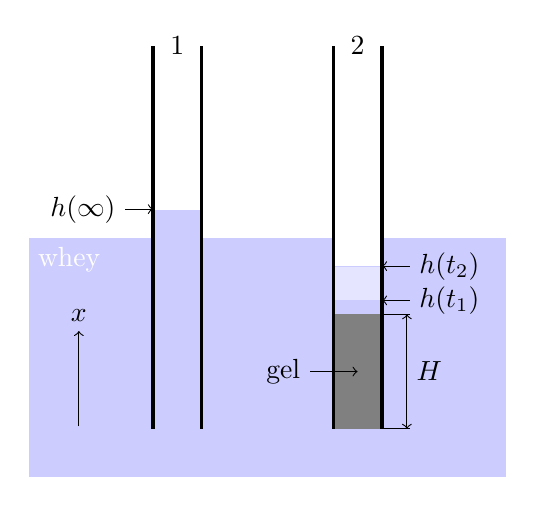
\begin{tikzpicture}
\node[minimum height=0.25\textwidth, minimum width=0.5\textwidth, fill=blue!20, anchor=north] (whey) at (0,0) {};
\begin{scope}[every node/.style={minimum width=0.05\textwidth}]
%where the tubes will be
\node[minimum height=0.4\textwidth, anchor=west] (tubel) at ($(whey.north)+(-0.12\textwidth,0)$) {};
\node[minimum height=0.4\textwidth, anchor=east] (tuber) at ($(whey.north)+(0.12\textwidth,0)$) {};
%Jurin in tubel
\node[minimum height=2em, anchor=west, fill=blue!20] (wheyinfty) at (tubel.west)  {};
%lack of liquid at t2
\node[minimum height=1em, anchor=north east, fill=white] (wheyt2) at (tuber.east) {};
%lack of liquid at t1
\node[minimum height=\baselineskip, anchor=north, fill=blue!10] (wheyt1) at (wheyt2.south) {};
\end{scope}
%gel
\fill[gray] (wheyt1.south west) +(0,-0.5em) rectangle (tuber.south east);
%draw tubes
\draw[very thick] (tubel.south west) -- (tubel.north west) (tubel.south east) -- (tubel.north east)
(tuber.south west) -- (tuber.north west) (tuber.south east) -- (tuber.north east);

%labels
\draw[<-] (wheyinfty.north west) -- +(-1em,0) node[left]{$h(\infty)$};
\draw[<-] (wheyt2.south east) -- +(1em,0) node[right]{$h(t_2)$};
\draw[<-] (wheyt1.south east) -- +(1em,0) node[right]{$h(t_1)$};
\draw  (wheyt1.south east) ++(0,-0.5em) -- +(1em,0) coordinate[pos=0.9] (Ht) (tuber.south east) -- +(1em,0) coordinate[pos=0.9] (Hb);
\draw[<->] (Ht) -- (Hb) node[midway, right] (H) {$H$};
\draw[<-] (H -| tuber) -- +(-0.05\textwidth,0) node[left]{gel};
\node[text=white,anchor=north west] at (whey.north west) {whey};
\node at (tubel.north) {$1$};
\node at (tuber.north) {$2$};
\draw[->] (whey.south west) ++(45:0.075\textwidth) -- +(0,0.1\textwidth) node[above] {$x$};
\end{tikzpicture}
\caption{Schematic representation of permeability measurement.}
\label{fig:tubexp}
\end{figure}
By measuring the liquid flux, $v$, of usually whey through open glass tubes filled with casein gels, the permeability coefficient, $B$, could be calculated from the known pressure gradient, $\nabla P$, according to equation \ref{eq:Darcy}. The apparatus used was developed by Van Dijk (1982) for measurements on rennet gels. Glass tubes open at both ends with an inner diameter of \SI{3.7}{\milli\metre} and a length of \SI{25}{\centi\metre} were placed in a precooled vat. The tubes placed in a holder rested on a plexiglass base. Acidified skimmilk or sodium caseinate was added to the vat to such an extent that the tubes were filled over a length of about \SI{10}{\centi\metre}. The gelation vat was heated according to the procedure given in section 2.3 (see original thesis). After the required gelation time at the appropriate temperature the tubes were with- drawn from the gelation vat, cleaned at the outside and placed in a rack, which was placed in the measuring vat made of clear plexiglass. The level of the percolating liquid in the measuring vat (usually whey or a sodium phosphate solution) was adjusted in such a way that the initial pressure gradient was about \SIrange{4.5e3}{6.0e3}{\pascal\per\metre}. The whey level in the tubes was read at regular time intervals with the help of a travelling microscope. The length of the intervals depended on the permeability of the gel matrix. From the five readings usually made four permeability coefficients could be calculated. The order of magnitude of the flow velocity, $v$, varied from \SIrange{3e-6}{8e-8}{\metre\per\second}. Assuming a value of \SI{1e-7}{\metre} for the parameter $\delta$ (i.e. a low estimate of the approximate diameter of casein particles) in eq.~\ref{eq:Reynolds} while $\rho\simeq \SI{1e3}{\kilo\gram\per\cubic\metre}$ and $\eta \simeq \SI{1e-3}{\pascal\second}$, the Reynolds number, $Re$, for the flow through casein gels varied from \SIrange{8e-9}{3e-7}{}. Taking for $\delta$ a pore diameter of \SIrange{1e-6}{1e-5}{\metre} instead of a particle diameter of \SI{1e-7}{\metre}, $Re$ will be 10 to 100 times larger, but still sufficiently small. There was therefore no risk for turbulent flow in our experiments. Variation of the pressure gradient from \SIrange{4.0}{11.0e3}{\pascal\per\metre} did not influence the calculated permeability coefficients, so that the application of Darcy's law for flow through acid casein gels seems allowable.

The calculation of $B$ from the experimental readings is somewhat complicated, because the pressure gradient is changing with time as the whey level in the glass tubes rises (see fig.~\ref{fig:tubexp}). On the other hand because of the rather homogeneous character of the gel and the one dimensional direction of flow (x-direction) the pressure gradient at a certain moment is constant and negative over the whole gel and is given by:
\begin{equation}
\frac{dP}{dx}(t) = -\rho g\frac{h(\infty)-h(t)}{H}
\end{equation}
\begin{description}
\item[$h(\infty)$] hight of the whey level in the reference tube (\si{\metre})
\item[$h(t)$] height of the whey level in the gel tube (\si{\metre})
\item[$H$] length of the casein gel (\si{\metre})
\item[$g$] gravitational acceleration (\si{\metre\per\square\second})
\end{description}

Because of the large volume outside the tubes $h(\infty)$ is assumed to be constant. The liquid flux, $v$, also changes with time:
\begin{equation}
v(t) = \frac{dh}{dt}(t)
\end{equation}

In this case the equation of Darcy (eq.~\eqref{eq:Darcy}) can be rewritten as:
\begin{equation}
 v(t) = \frac{dh}{dt}(t) = \frac{B}{\eta}\rho g\frac{h(\infty)-h(t)}{H}
\end{equation}

Integration, solving the integration constant and rewriting leads to an expression for $B$, depending on $h(t)$ at $t=t_1$ and $t=t_2$ (Van Dijk, 1982).
\begin{equation}
B = -\frac{\eta H \ln\left(\frac{h(\infty)-h(t_2)}{h(\infty)-h(t_1)}\right)}{\rho g (t_2-t_1)}
\end{equation}

Within the experimental accuracy the permeability coefficient, $B$, of acid casein gels did not change with time during the experiment.


\end{document}